\chapter{Implementation}
\label{ch:implementation}

This chapter details the Python implementation of our hybrid retrieval system, describing the architectural decisions, core components, and practical trade-offs made to deliver a working system within banking infrastructure constraints.

\section{Project Structure}

The implementation follows a modular architecture with clear separation between user interface components, retrieval logic, and data management:

\begin{lstlisting}[language=bash, caption={Project directory structure}, label={lst:project-structure}]
validation-rule-search/
├── app.py                 # Main Dash application entry point
├── config.py             # Configuration settings
├── requirements.txt      # Python dependencies
├── components/           # UI Components
│   ├── generator.py     # Chat interface UI
│   ├── search.py       # Search interface with filters
│   └── layout.py       # Unified interface
├── rag/                 # Retrieval-Augmented Generation
│   ├── embeddings/     # Embedding management
│   │   ├── manager.py # Model operations
│   │   └── index.py   # Semantic search
│   └── search/        # Search implementation
│       └── retriever.py # Hybrid retrieval
├── db/                 # Database layer
│   ├── manager.py     # SQLite operations
│   └── rules.db       # Generated database
└── data/
    └── validation_rules.csv # Standardized corpus
\end{lstlisting}

\section{System Architecture}

The system implements a monolithic architecture optimized for banking deployment constraints. All components run within a single Dash application process, sharing memory-efficient data structures and eliminating network overhead. Figure~\ref{fig:callback-map} illustrates the callback architecture showing data flow between UI components and the retrieval engine.

\begin{figure}[!htbp]
\centering
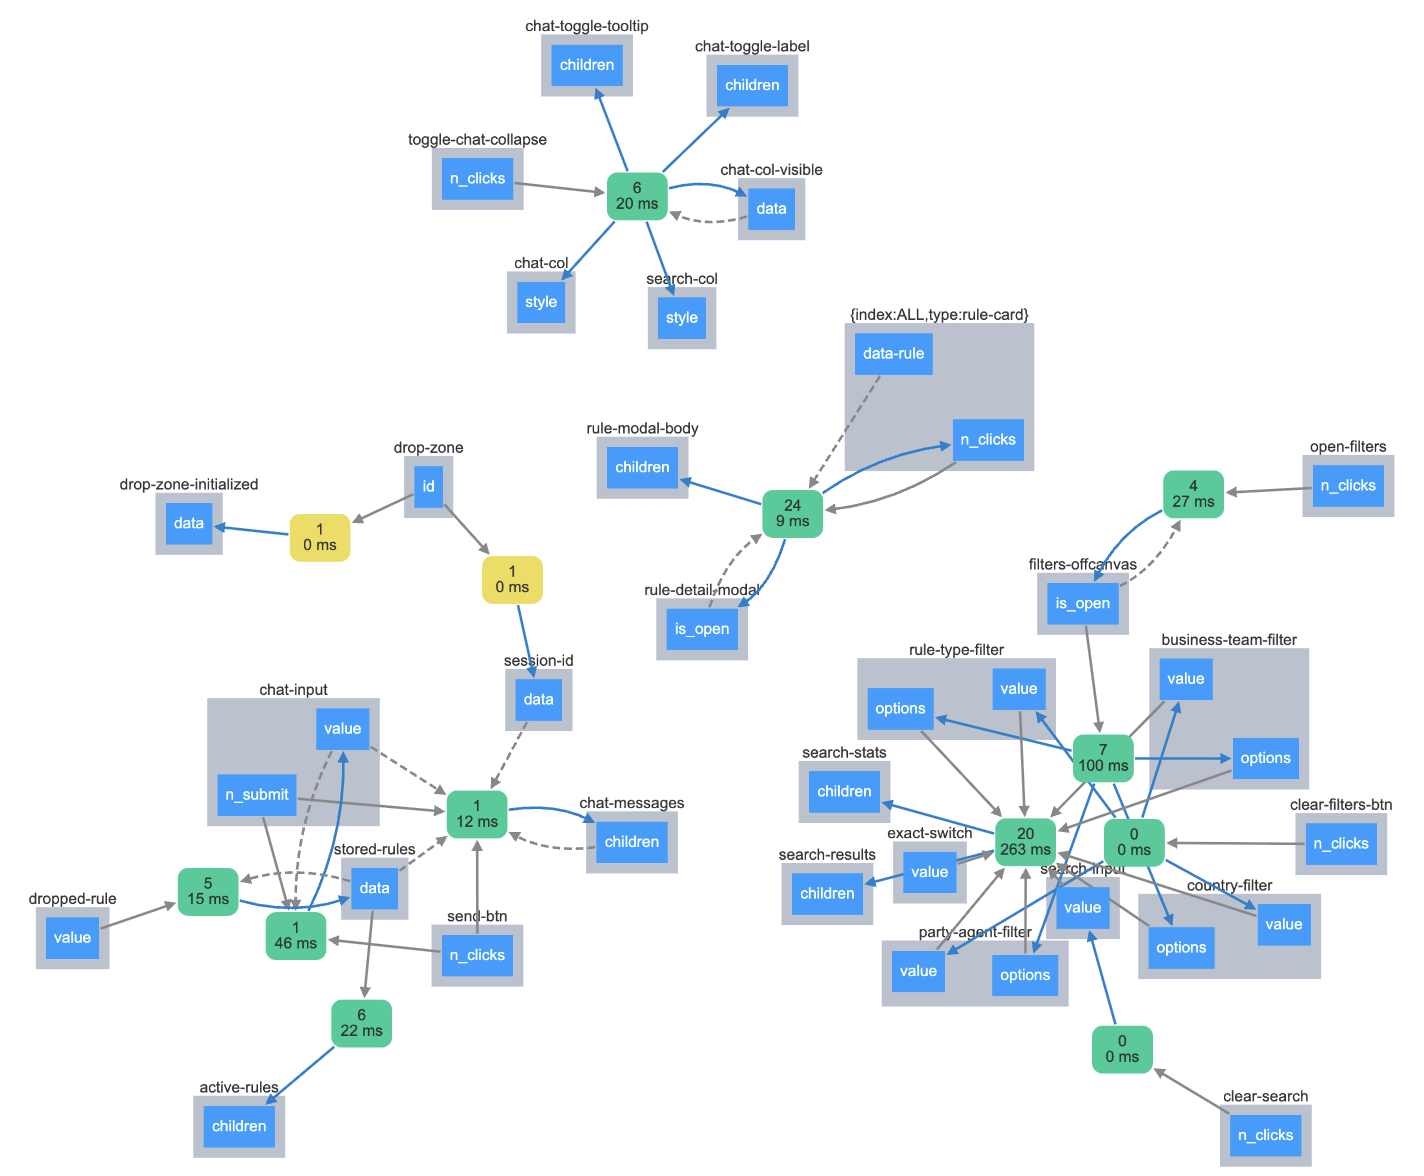
\includegraphics[width=0.85\textwidth]{Figures/callback_map.png}
\caption{Callback architecture showing data flow between UI components and retrieval engine.}
\label{fig:callback-map}
\end{figure}

\subsection{Core Dependencies}

The system uses established Python libraries, minimizing external dependencies:

\begin{table}[!htbp]
\centering
\small
\begin{tabular}{lll}
\toprule
\textbf{Library} & \textbf{Version} & \textbf{Purpose} \\
\midrule
dash & 2.18.2 & Web application framework \\
pandas & 2.2.3 & Data processing \\
numpy & 1.26.0 & Numerical operations \\
scikit-learn & 1.6.1 & Similarity computation \\
rank-bm25 & 0.2.2 & Keyword matching \\
fuzzywuzzy & 0.18.0 & String similarity \\
transformers & 4.48.0 & HuggingFace models \\
torch & 2.2.2 & Neural networks \\
\bottomrule
\end{tabular}
\caption{Core Python dependencies.}
\label{tab:impl-dependencies}
\end{table}

\section{Application Bootstrap}

The system follows a deterministic initialization sequence ensuring robust startup:

\begin{lstlisting}[language=Python, caption={Bootstrap sequence (app.py)}, label={lst:bootstrap}]
def boot() -> tuple[dash.Dash, RuleRetriever]:
    """Initialize application components."""
    app = create_app()
    
    # Database initialization
    db_manager = DatabaseManager(
        db_path="db/rules.db",
        table_name="rules"
    )
    db_manager.init_db("data/validation_rules.csv")
    
    # Retriever with tuned weights
    config = SearchConfig(
        semantic_weight=0.80,  # LOOCV-tuned
        bm25_weight=0.10,
        fuzzy_weight=0.10,
        min_similarity=0.30    # Semantic gate
    )
    
    retriever = RuleRetriever(
        embedding_manager=EmbeddingManager(),
        config=config,
        db_manager=db_manager
    )
    
    # Register UI callbacks
    register_callbacks(app, retriever)
    return app, retriever
\end{lstlisting}

\section{User Interface Implementation}

The UI provides dual interfaces for search and generation, unified in a responsive layout. The implementation uses Dash with Bootstrap components for a modern, professional appearance.

\subsection{Search Interface}

The search component offers faceted filtering and hybrid retrieval modes. As shown in Figure~\ref{fig:search-interface}, the interface includes natural language query input with debouncing, toggle between Keyword and Hybrid search modes, and real-time result updates as filters change.

\textbf{Interaction Modes:}

The system supports three distinct interaction modes to accommodate different user workflows:

\begin{itemize}[leftmargin=*,itemsep=2pt,topsep=2pt]
  \item \textbf{Search mode}: Query-driven retrieval with relevance ranking based on hybrid scoring
  \item \textbf{Browse mode}: Filter-based exploration where users can view all rules matching specific criteria without entering a query
  \item \textbf{Filtered search}: Query execution within a pre-filtered subset, combining both approaches
\end{itemize}

When no query is provided, filtered rules receive a score of 1.0, indicating perfect match to the filter criteria. This design choice ensures that users can explore the rule corpus by category even without knowing specific search terms—particularly valuable for QA teams reviewing all rules for a specific country or validation type.

\begin{figure}[!htbp]
\centering
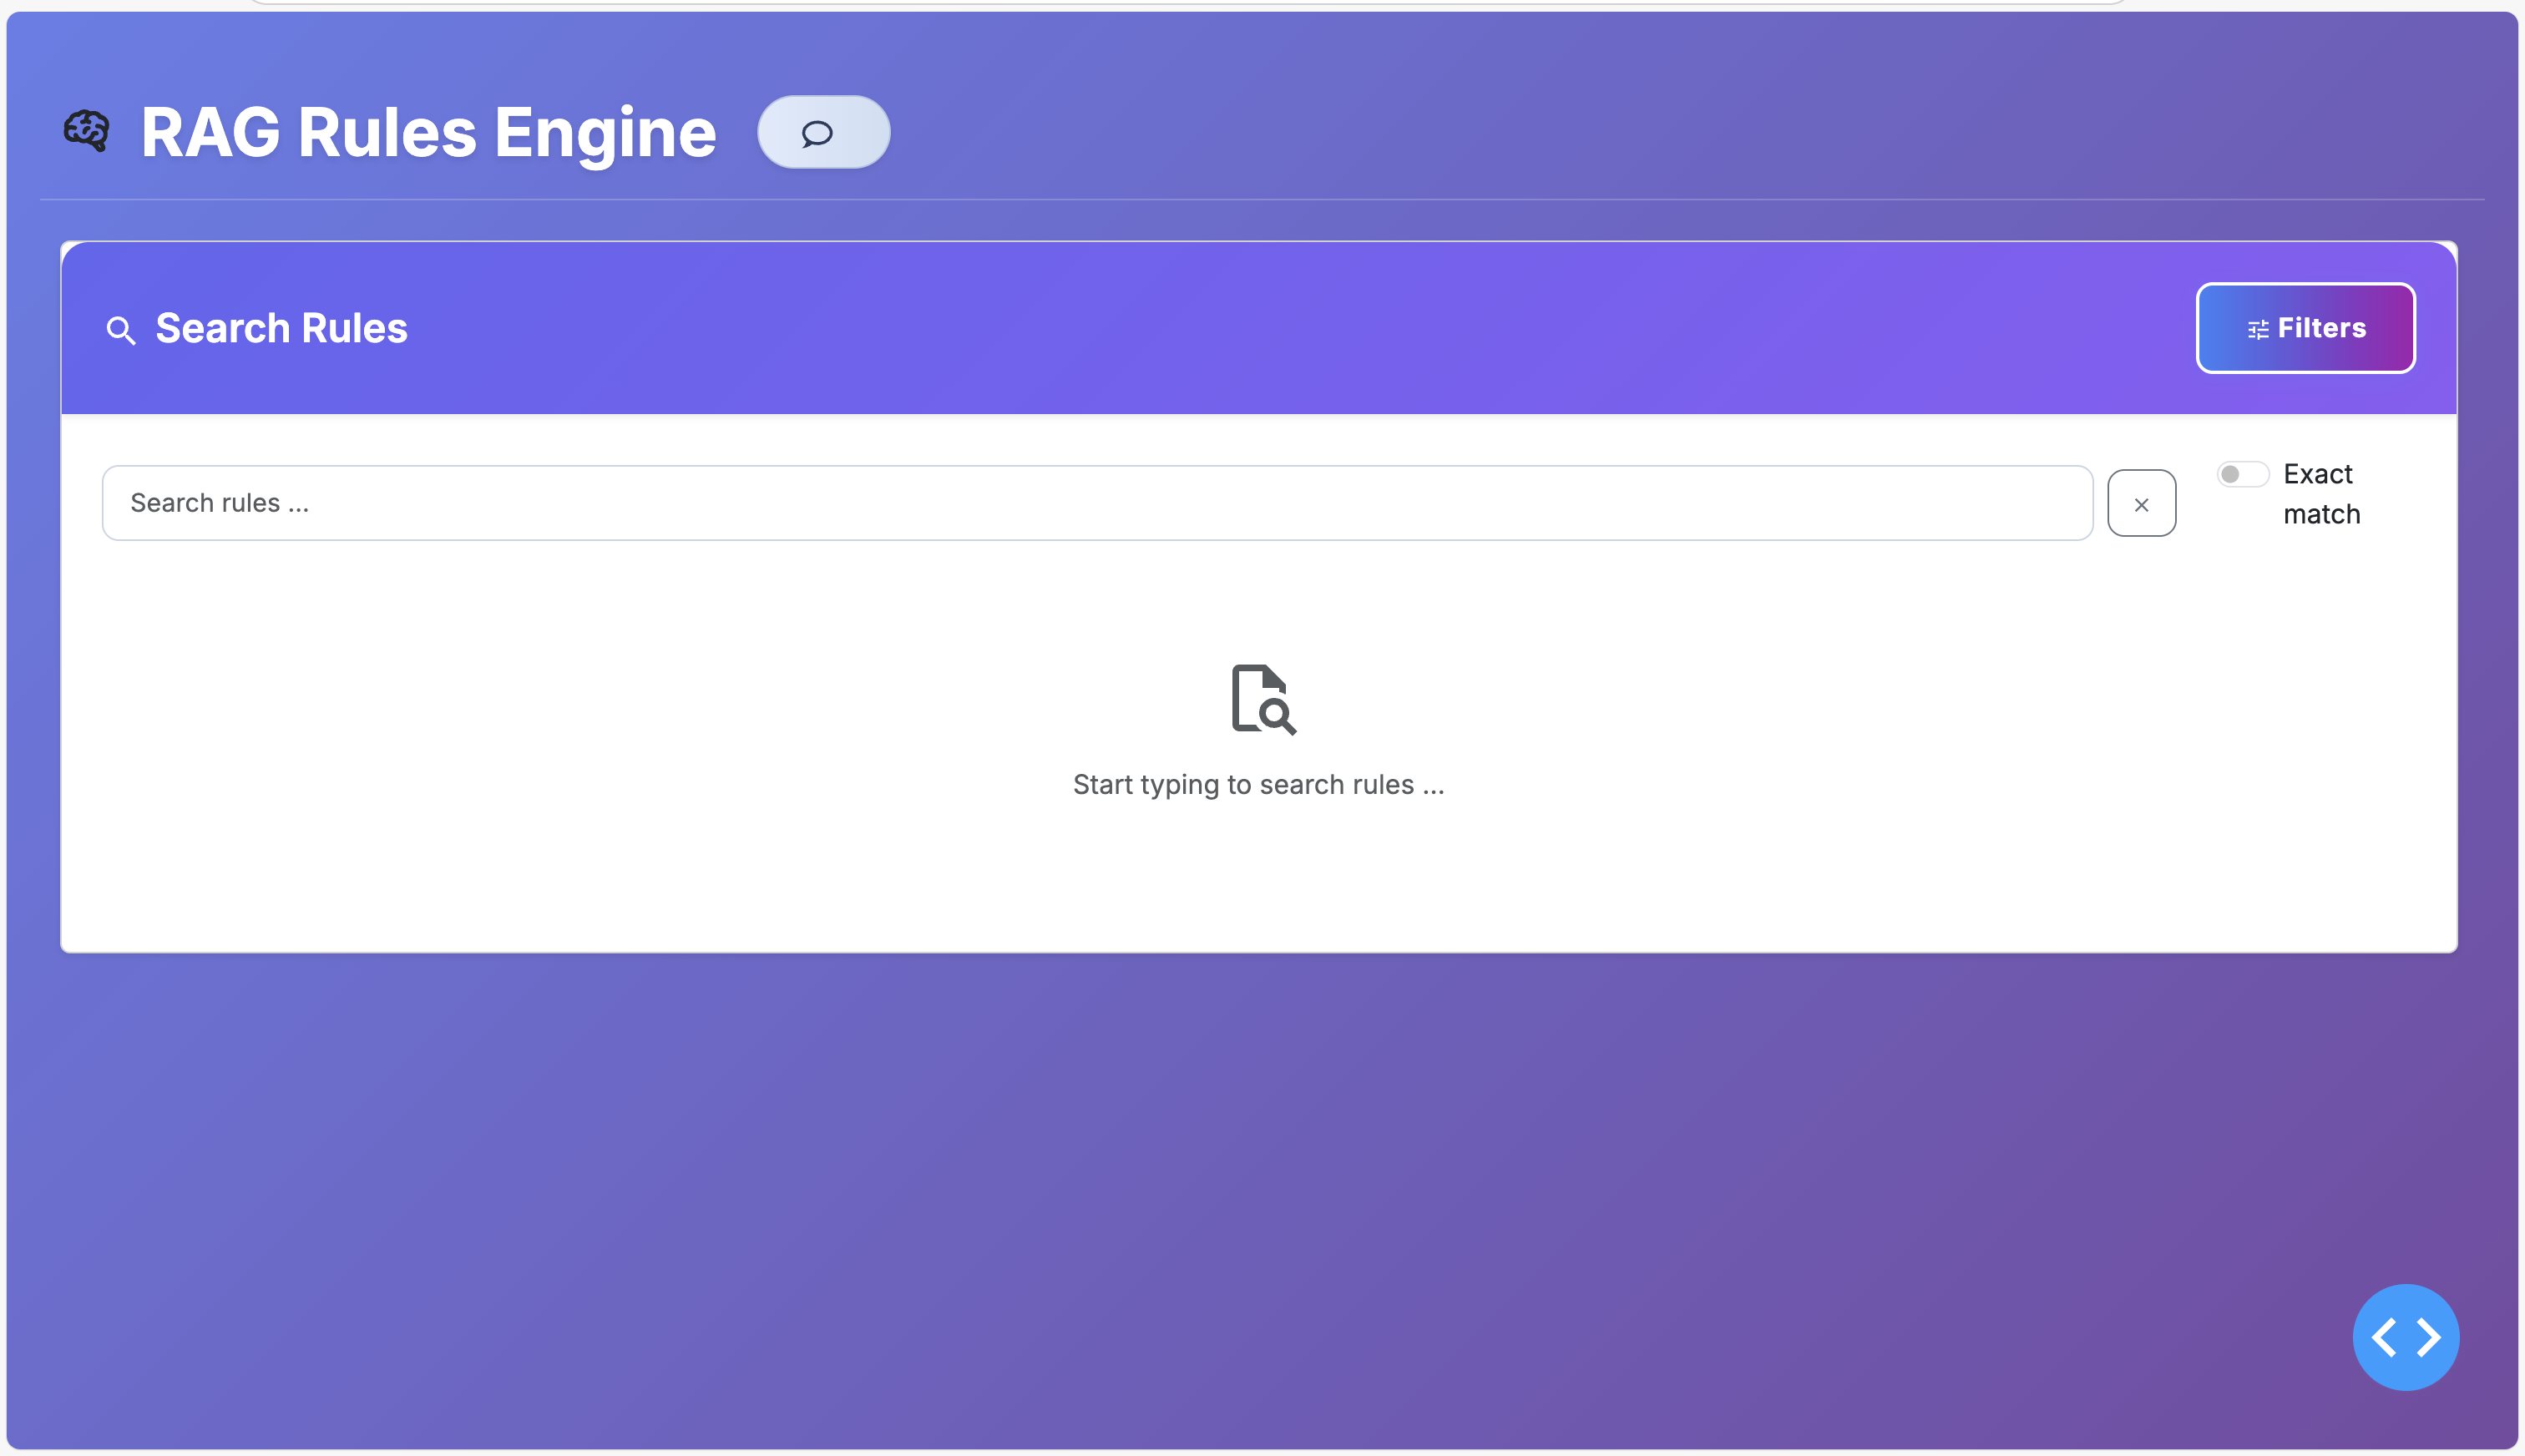
\includegraphics[width=0.9\textwidth]{Figures/full_search.png}
\caption{Search interface with query input, filters panel, and mode selection.}
\label{fig:search-interface}
\end{figure}

\subsection{Faceted Filtering}

The system provides multi-select dropdowns for categorical refinement across Rule Type, Country, Business Type, and Party Agent dimensions, as illustrated in Figure~\ref{fig:search-filters}.

\begin{figure}[!htbp]
\centering
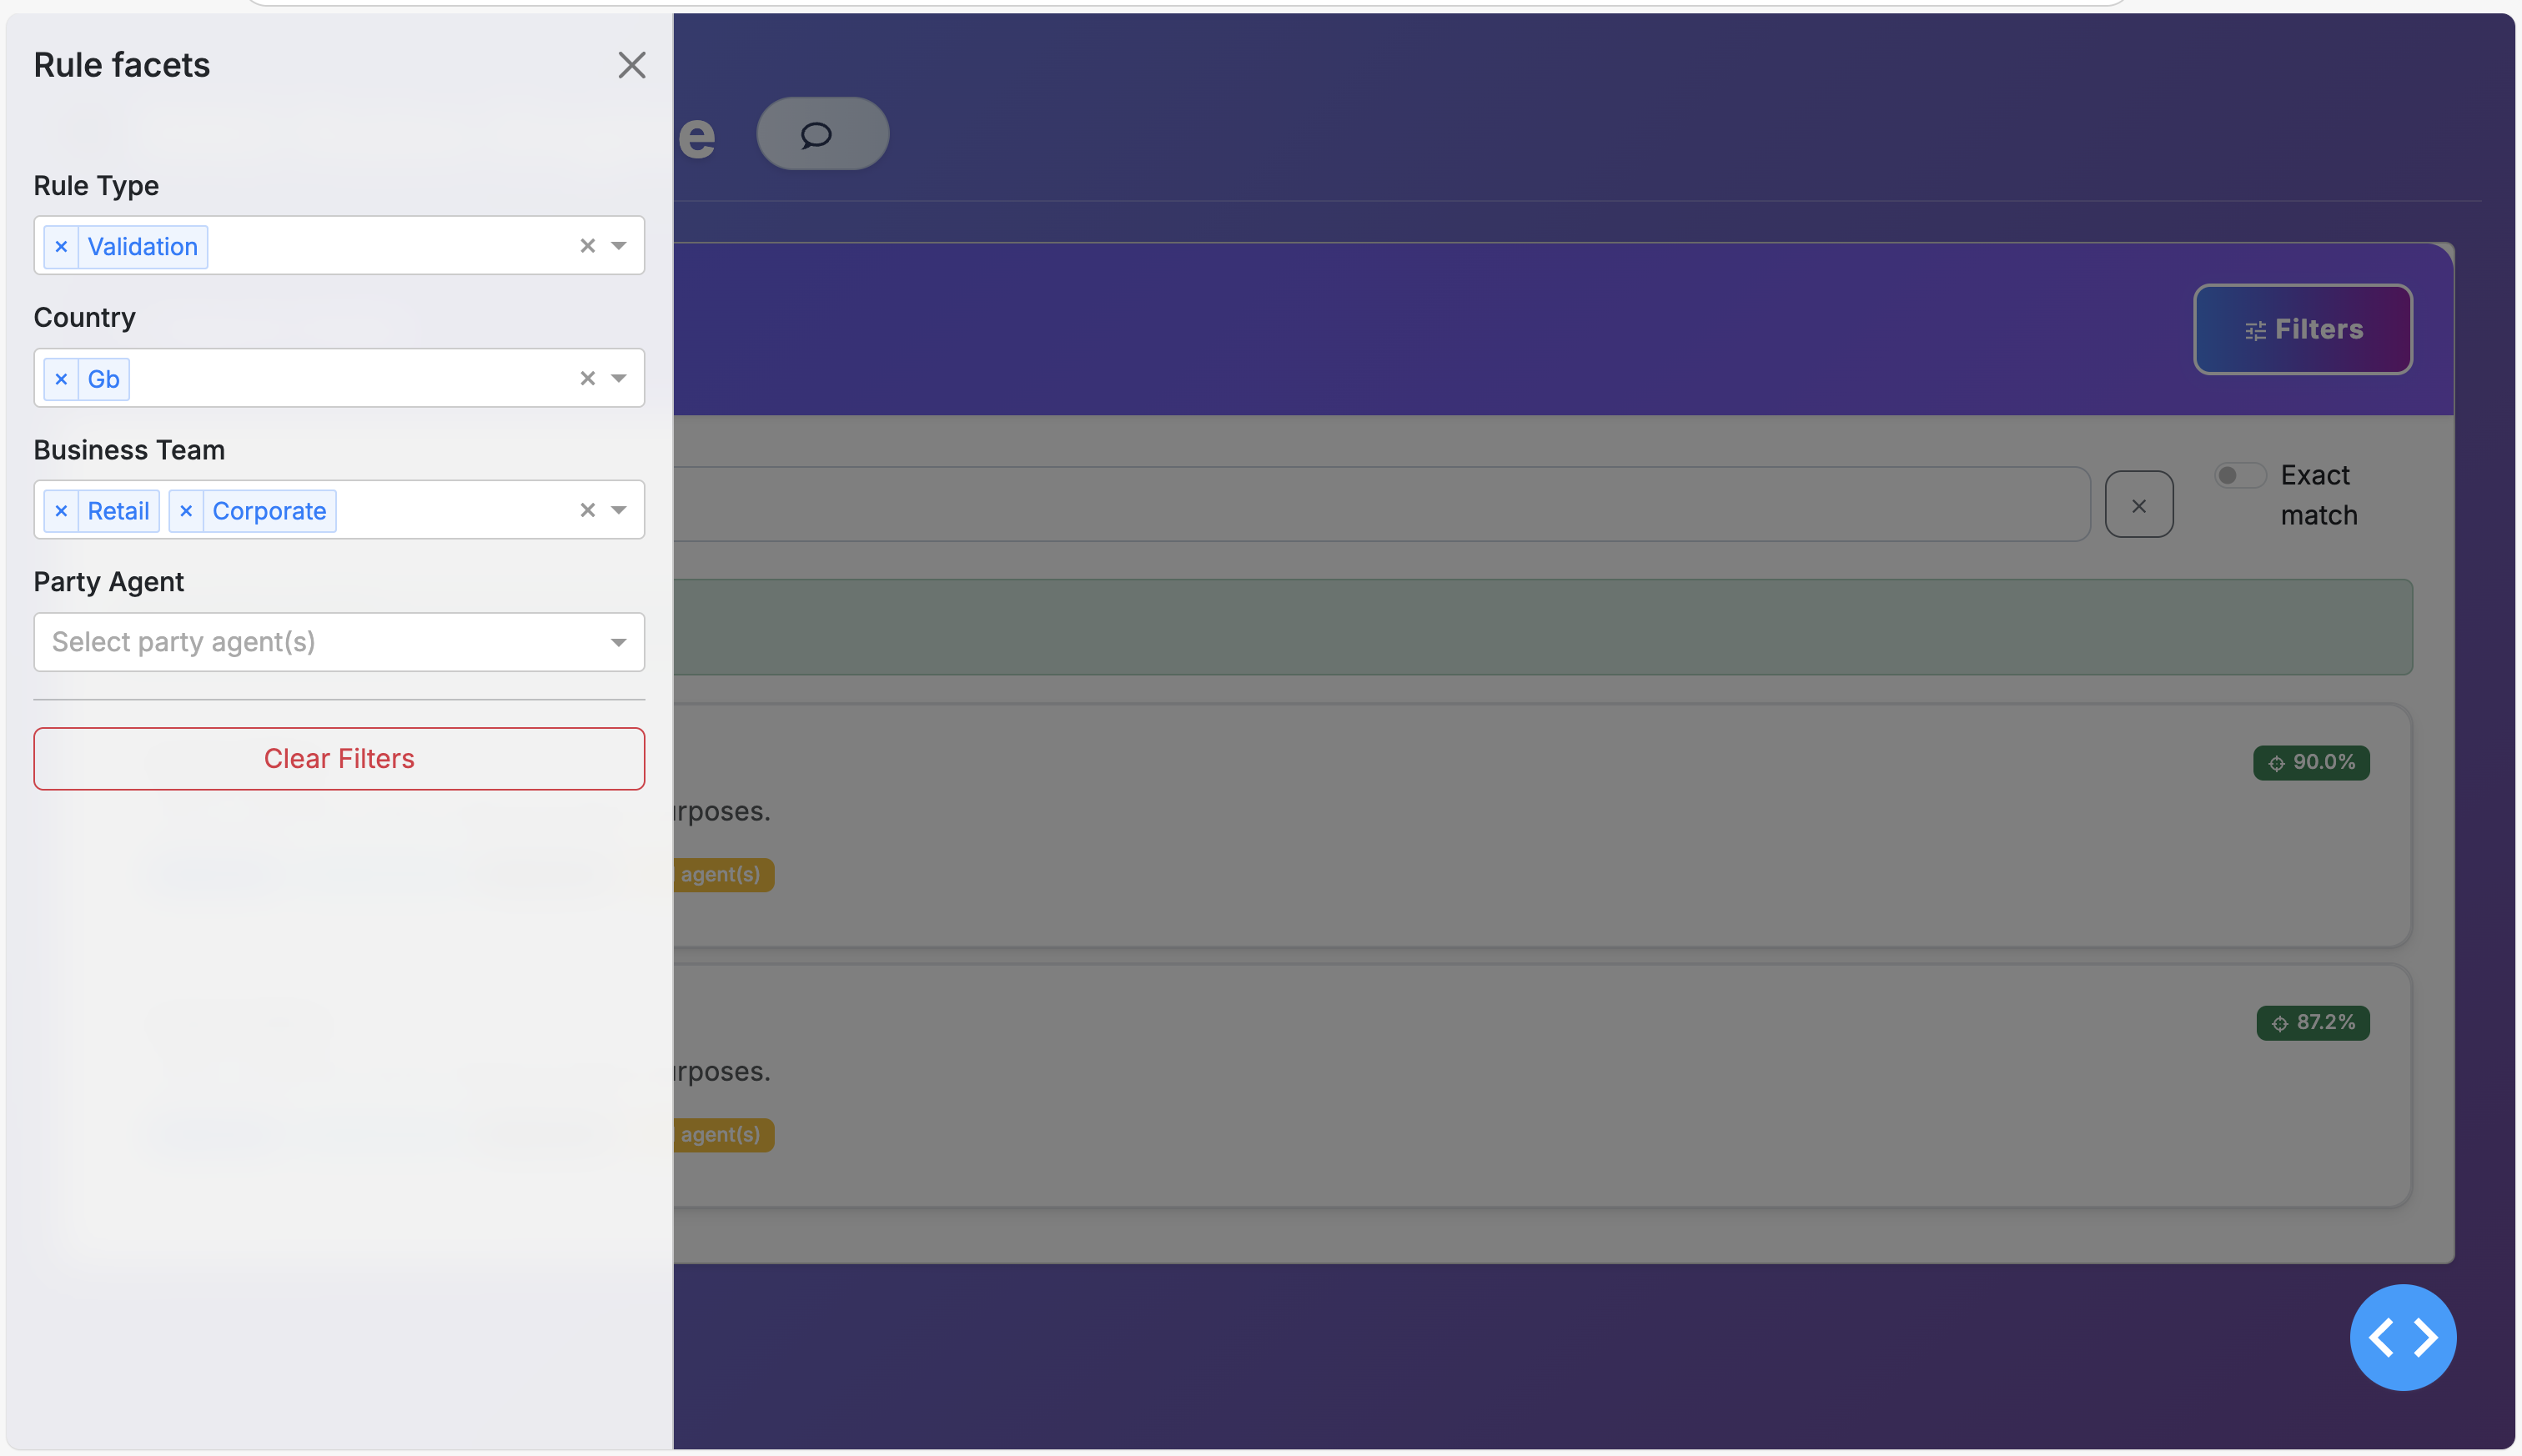
\includegraphics[width=0.9\textwidth]{Figures/search_filters.png}
\caption{Faceted filtering panel showing multi-select dropdowns for categorical refinement.}
\label{fig:search-filters}
\end{figure}

\subsection{Search Results and Details}

Results are presented as interactive cards with similarity scores and metadata badges. Each card is draggable for interaction with the generator component. Figure~\ref{fig:search-results} shows the result display format.

\begin{figure}[!htbp]
\centering
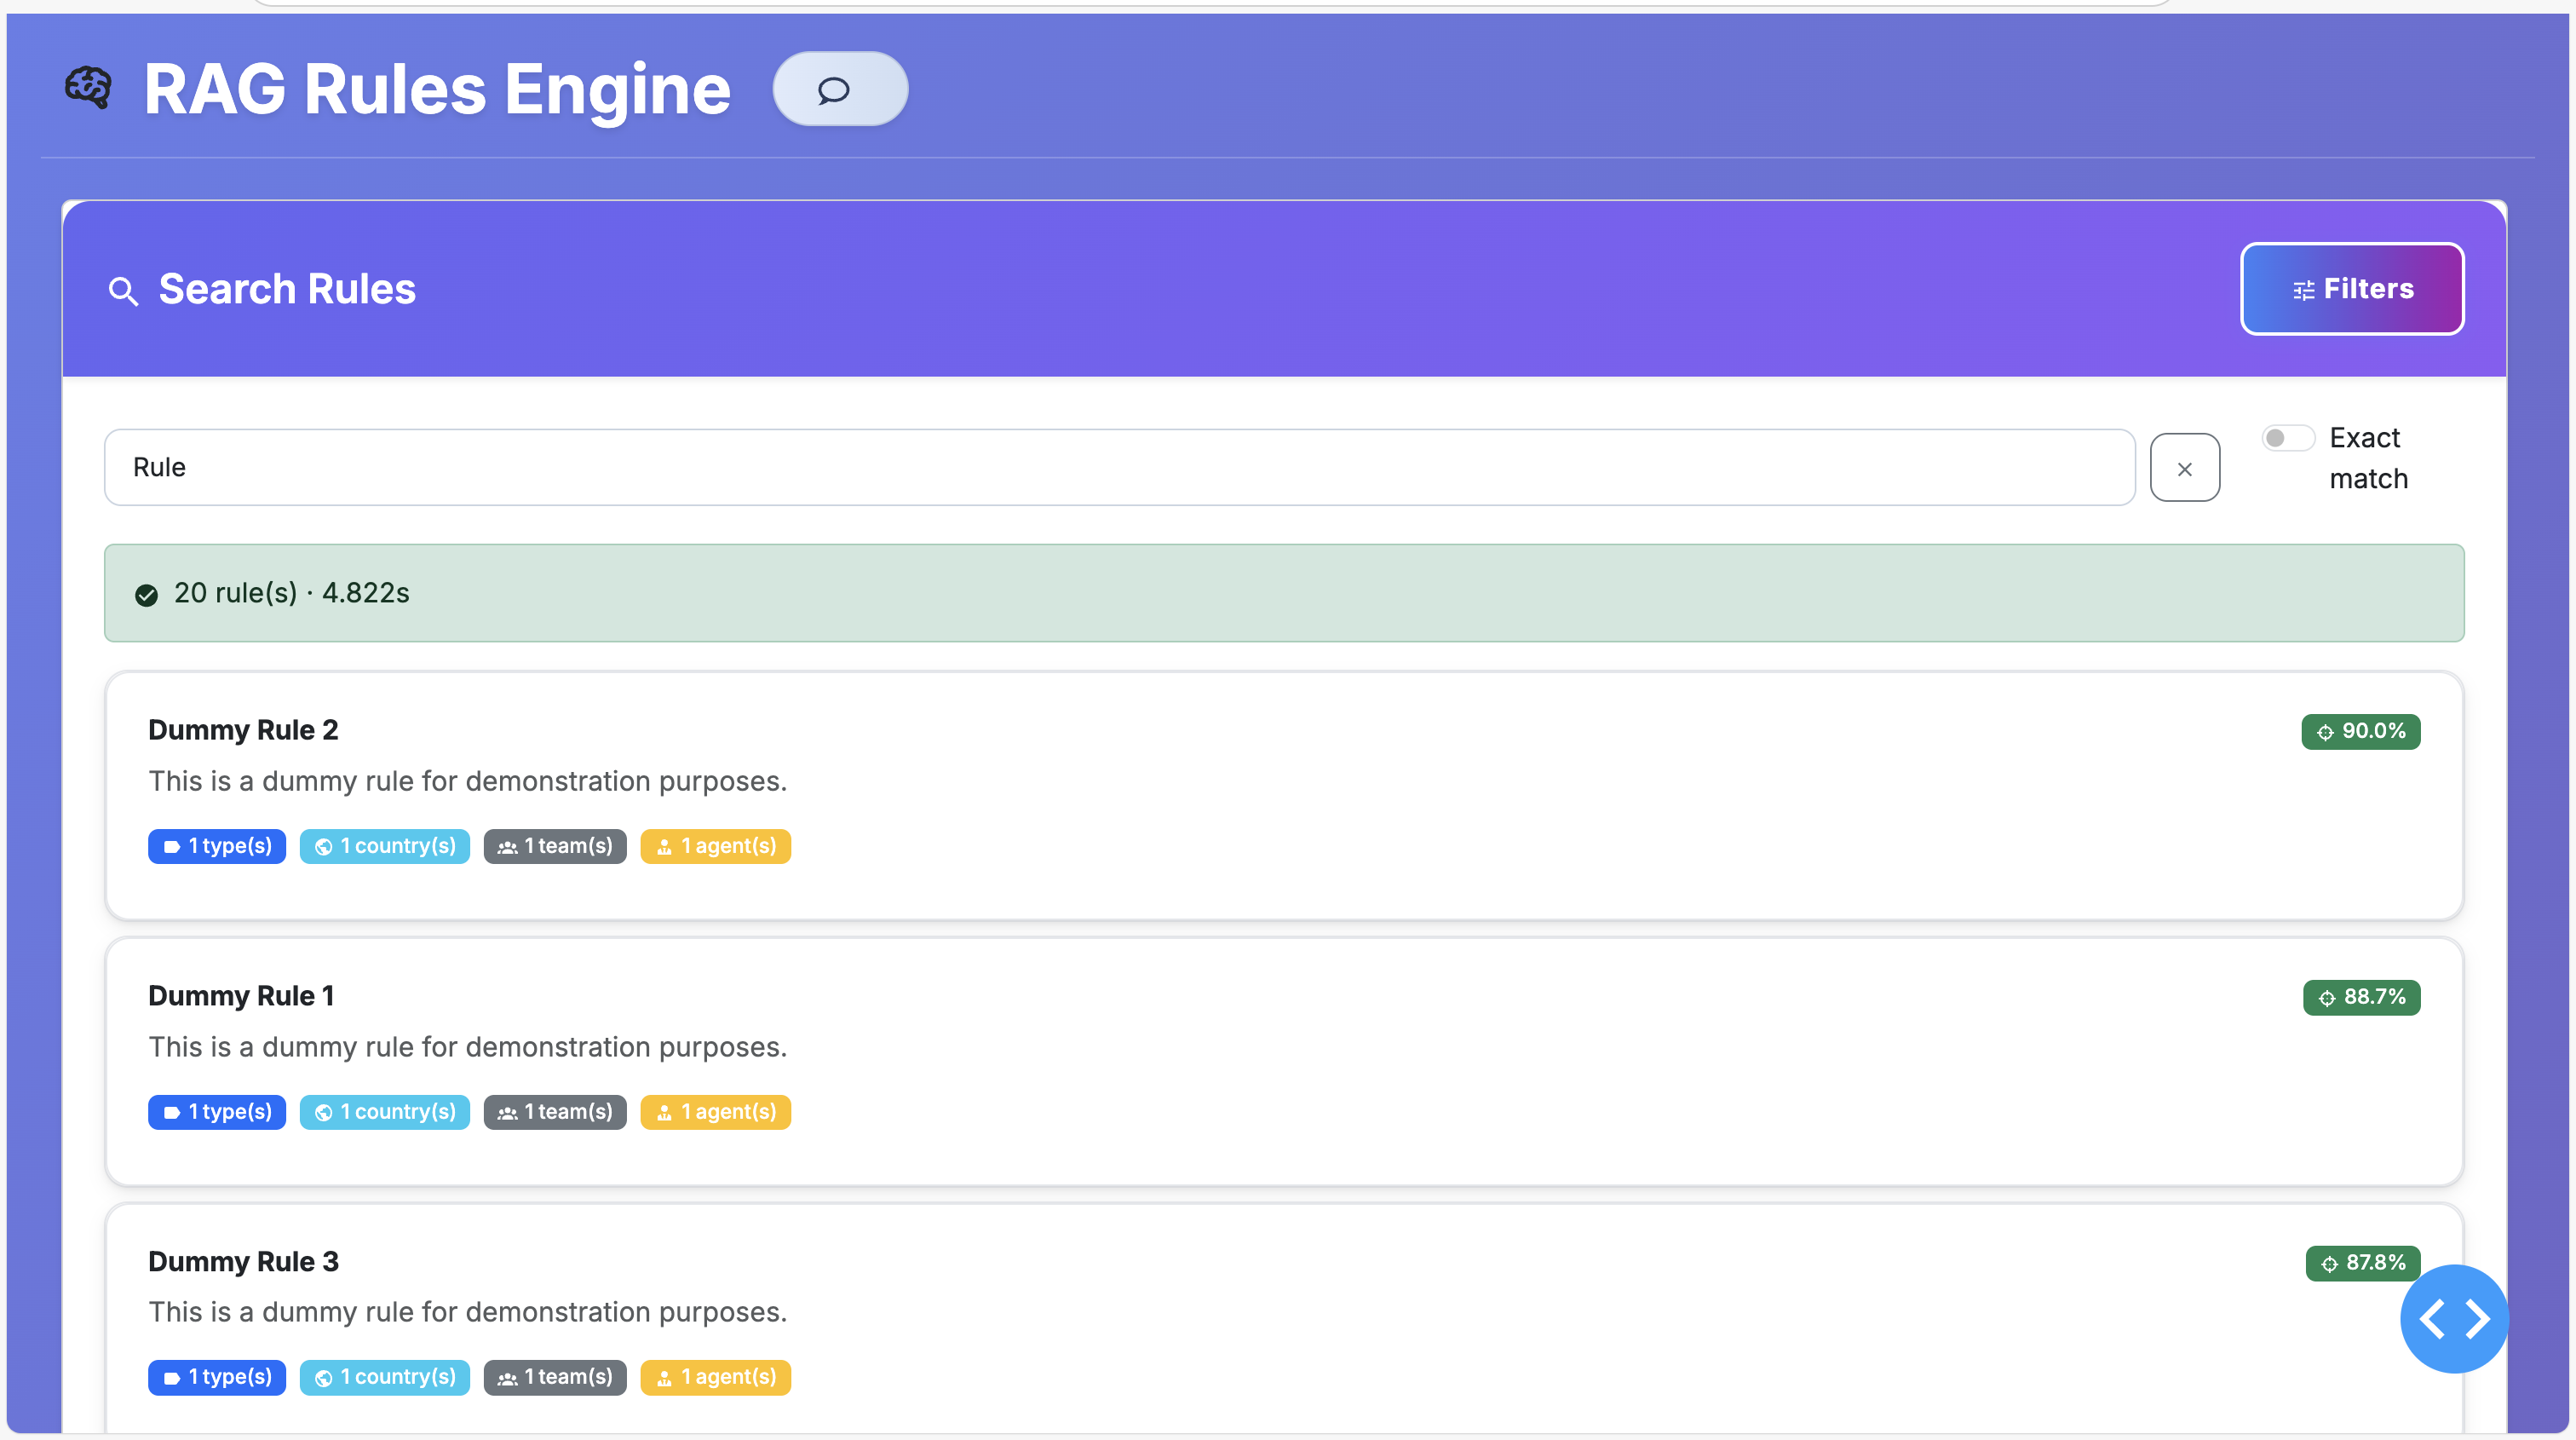
\includegraphics[width=0.9\textwidth]{Figures/full_search_results.png}
\caption{Search results showing ranked rule cards with similarity scores and metadata badges.}
\label{fig:search-results}
\end{figure}

Clicking a rule card opens a detailed modal (Figure~\ref{fig:rule-details}) displaying complete rule information including Kotlin code, descriptions, error codes, and metadata tags.

\begin{figure}[!htbp]
\centering
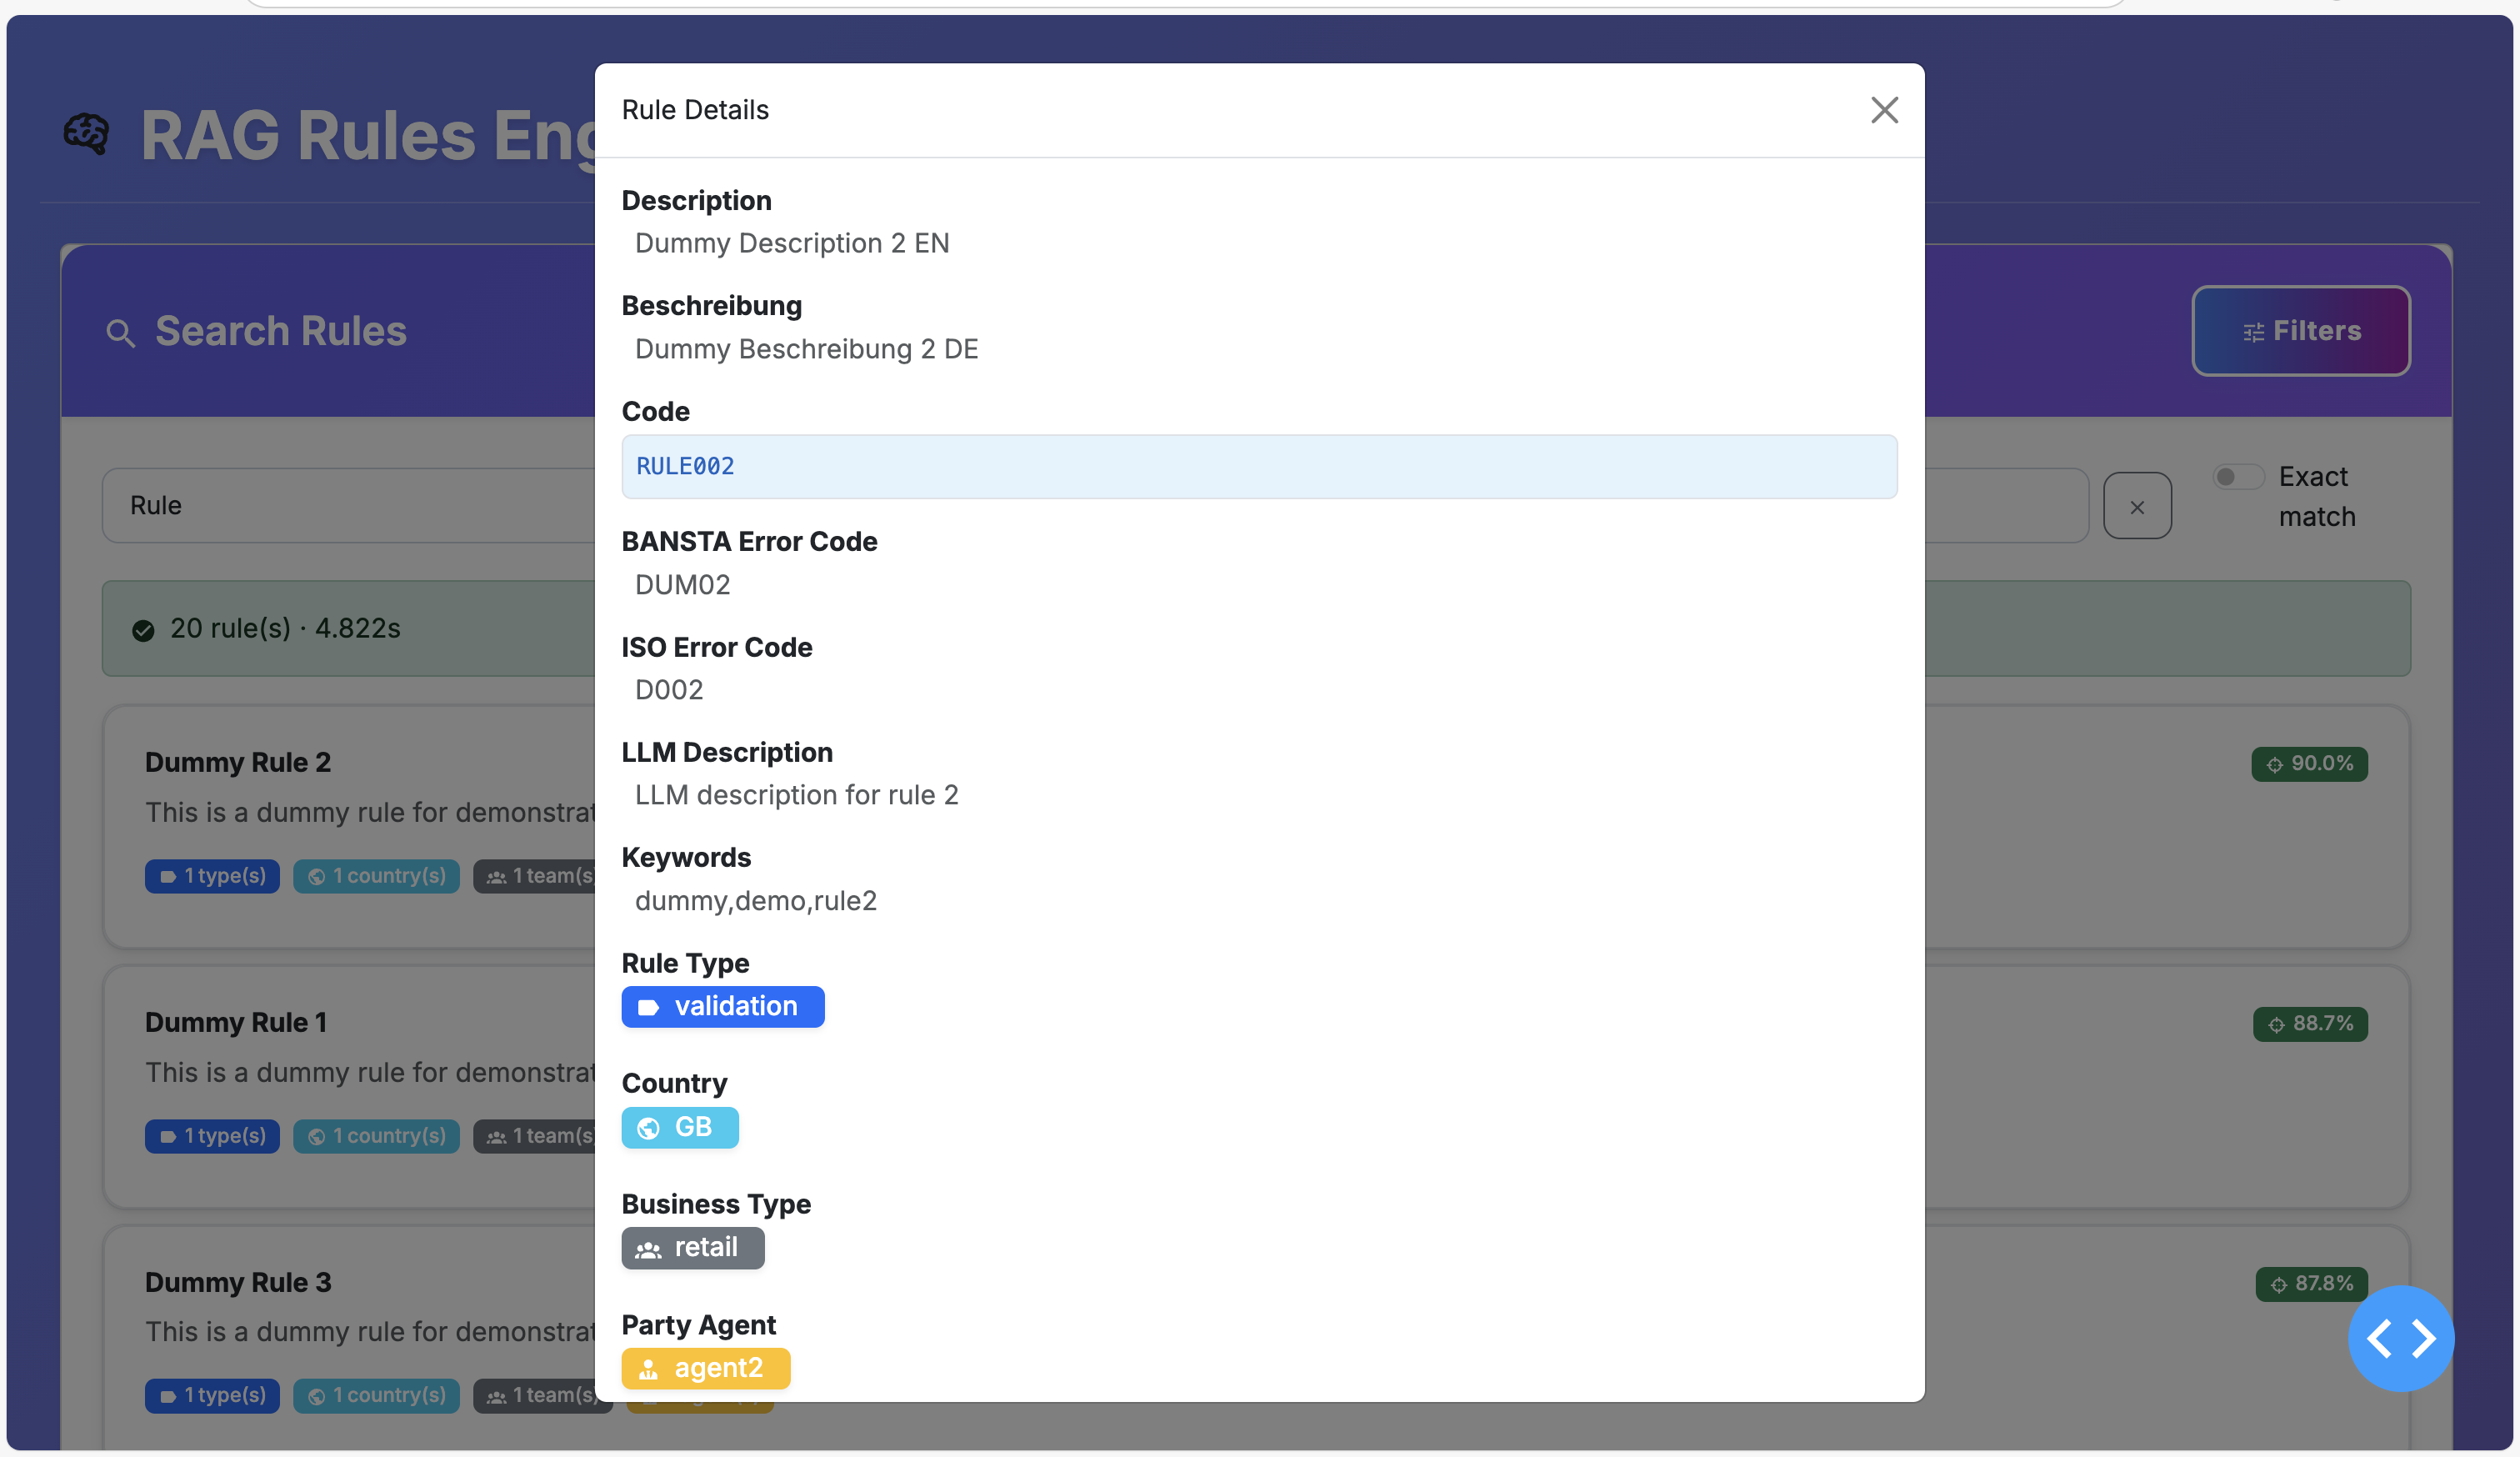
\includegraphics[width=0.85\textwidth]{Figures/rule_details.png}
\caption{Rule detail modal displaying complete rule information.}
\label{fig:rule-details}
\end{figure}

\subsection{Integrated Chat Interface}

The system supports conversational interaction alongside traditional search, as demonstrated in Figure~\ref{fig:search-chat}. Users can drag rules from search results into the chat context for detailed exploration.

\begin{figure}[!htbp]
\centering
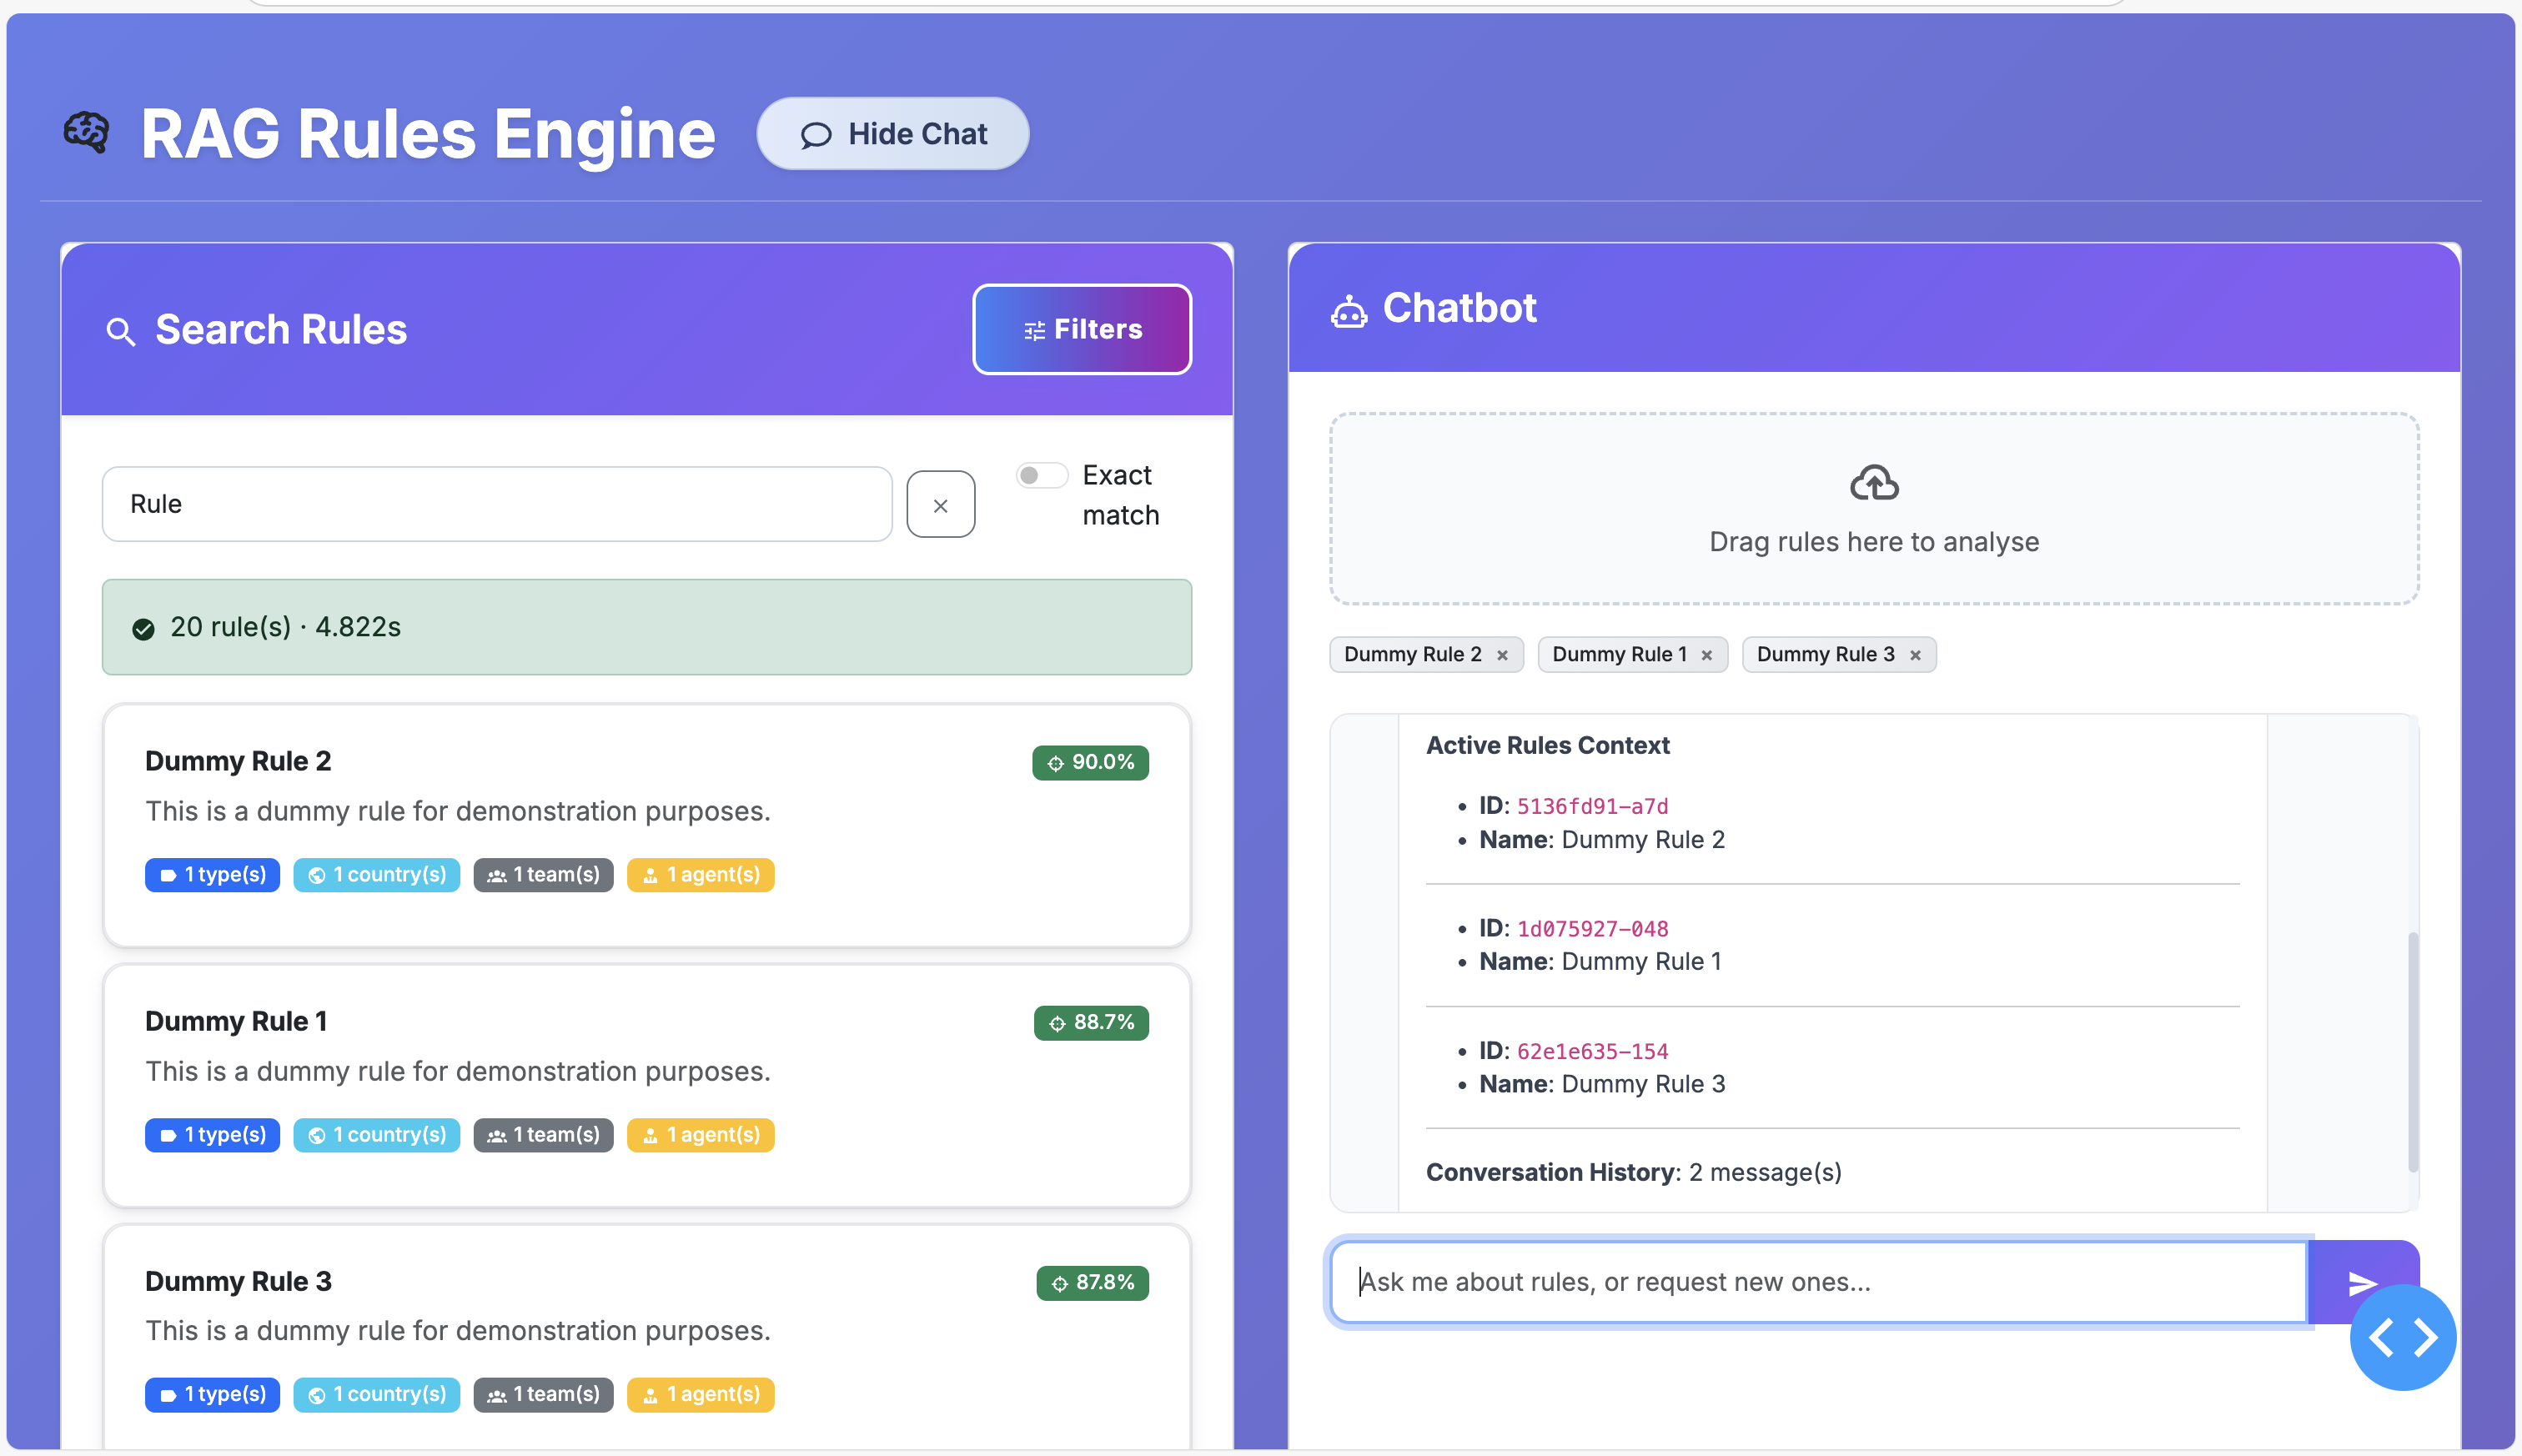
\includegraphics[width=0.95\textwidth]{Figures/search_chat_example.png}
\caption{Unified interface showing search results (left) and chat-based rule exploration (right).}
\label{fig:search-chat}
\end{figure}

\section{Core Retrieval Components}

\subsection{Embedding Management}

The embedding manager handles UAE-Large-V1 model operations with attention-aware pooling:

\begin{lstlisting}[language=Python, caption={Mean pooling implementation for embeddings}, label={lst:mean-pooling}]
def _mean_pooling(self, model_output, attention_mask):
    """Attention-mask-aware mean pooling."""
    token_embeddings = model_output.last_hidden_state
    mask = attention_mask.unsqueeze(-1)
    
    # Sum only non-padding tokens
    sum_embeddings = (token_embeddings * mask).sum(dim=1)
    token_counts = mask.sum(dim=1).clamp(min=1e-9)
    
    return sum_embeddings / token_counts
\end{lstlisting}

This implementation ensures that padding tokens do not affect the final embedding representation, providing accurate semantic representations for variable-length inputs.

\subsection{Hybrid Scoring}

The retriever implements per-query normalization with semantic gating:

\begin{lstlisting}[language=Python, caption={Hybrid score computation with semantic gate}, label={lst:hybrid-scoring}]
def _hybrid_scores(self, query, rules):
    """Weighted combination with semantic gate."""
    # Get raw scores from each signal
    sem_raw = self._semantic_scores(query, rules)
    bm25_raw = self._bm25_scores(query, rules)
    fuzzy_raw = self._fuzzy_scores(query, rules)
    
    # Per-signal normalization to [0,1]
    sem = self._normalize_per_prompt(sem_raw)
    bm25 = self._normalize_per_prompt(bm25_raw)
    fuzzy = self._normalize_per_prompt(fuzzy_raw)
    
    # Apply semantic gate (tau = 0.30)
    for rule_id in sem:
        if sem[rule_id] < 0.30:
            sem[rule_id] = 0.0
    
    # Weighted combination
    scores = {}
    for rule in rules:
        rid = rule["rule_id"]
        scores[rid] = (
            0.80 * sem.get(rid, 0.0) +
            0.10 * bm25.get(rid, 0.0) +
            0.10 * fuzzy.get(rid, 0.0)
        )
    
    return scores
\end{lstlisting}

\section{Performance Optimizations}

\subsection{Memory Management}

The implementation employs several strategies to minimize memory footprint:

\begin{itemize}[leftmargin=*,itemsep=3pt,topsep=3pt]
  \item \textbf{Float32 precision}: Reduces embedding memory by 50\% compared to float64
  \item \textbf{Lazy loading}: Embeddings parsed from JSON only when accessed
  \item \textbf{Shared arrays}: NumPy views prevent unnecessary copying
  \item \textbf{Result limiting}: Candidate pools capped at 100 rules
  \item \textbf{Garbage collection}: Explicit cleanup after batch operations
\end{itemize}

\subsection{Query Performance}

Query latency breakdown shows consistent sub-100ms performance:

\begin{table}[!htbp]
\centering
\begin{tabular}{lrr}
\toprule
\textbf{Operation} & \textbf{Time (ms)} & \textbf{Optimization} \\
\midrule
Filter application & 5 & SQLite indices \\
BM25 scoring & 20 & Pre-computed IDF \\
Fuzzy matching & 15 & Cached lowercasing \\
Semantic search & 10 & Matrix multiplication \\
Normalization & 5 & Vectorized operations \\
Hybrid scoring & 5 & NumPy broadcasting \\
Ranking & 2 & Partial sort \\
\midrule
\textbf{Total} & \textbf{62} & \textbf{Well within target} \\
\bottomrule
\end{tabular}
\caption{Query latency breakdown showing sub-100ms performance.}
\label{tab:query-performance}
\end{table}

\section{Configuration Management}

System configuration is centralized in a single file with clear parameter definitions:

\begin{lstlisting}[language=Python, caption={Configuration settings (config.py)}, label={lst:config}]
# Application settings
APP_TITLE = "Validation Rules Search Engine"
DEBUG = 1
HOST = "127.0.0.1"
PORT = 8050

# Search weights (LOOCV-tuned)
SEMANTIC_WEIGHT = 0.8
BM25_WEIGHT = 0.1
FUZZY_WEIGHT = 0.1

# Semantic gate threshold
MIN_SIMILARITY = 0.3

# Model configuration
EMBEDDING_MODEL = "models/embeddings/UAE-Large-V1"

# Database settings
SQLITE_DB_PATH = "db/rules.db"
CSV_DATA_PATH = "data/validation_rules.csv"
\end{lstlisting}

\section{Implementation Challenges}

Several challenges were encountered and resolved during implementation:

\subsection{Startup Latency}

\textbf{Challenge}: Building indices for 1,157 rules adds approximately 600ms to startup time.

\textbf{Solution}: Implemented parallel index construction using ThreadPoolExecutor, reducing initialization time by 40\%. Indices are built once at startup and reused for all queries.

\subsection{Memory Usage}

\textbf{Challenge}: Full-precision embeddings require 9.5MB for 1,157 rules.

\textbf{Solution}: Adopted float32 precision (4.7MB) and lazy loading from JSON storage. Embeddings are loaded once and shared across all requests using NumPy views.

\subsection{Database Concurrency}

\textbf{Challenge}: SQLite database locks under concurrent access patterns.

\textbf{Solution}: Configured WAL (Write-Ahead Logging) mode for concurrent reads, implemented busy timeout with retry logic, and minimized write operations after initialization.

\section{Summary}

The implementation successfully delivers a hybrid retrieval system within strict operational constraints. Through careful architectural decisions and practical optimizations, we achieve:

\begin{itemize}[leftmargin=*,itemsep=3pt,topsep=3pt]
  \item Complete functionality in approximately 2,500 lines of Python
  \item Sub-100ms query latency for typical searches
  \item Memory footprint under 256MB total
  \item Zero external dependencies beyond Python libraries
  \item Maintainable architecture with clear module boundaries
\end{itemize}

The system demonstrates that enterprise-grade retrieval can be achieved through thoughtful engineering within constraints, validating our hypothesis that complex infrastructure is not required when requirements are well-understood and constraints are properly addressed.
